\documentclass{article}
\usepackage[utf8]{inputenc}
\usepackage[margin=1in]{geometry}
\usepackage{mathptmx}
\usepackage{mathtools}
\usepackage{amsmath}
\usepackage{subcaption}
\setlength{\parindent}{0em}
\setlength{\parskip}{0.5em}


\title{All Figures in Assignment 3 - CTA200}
\author{Rishik Adhikari}
\date{May 11, 2023}

\usepackage{natbib}
\usepackage{graphicx}

\begin{document}

\maketitle

\begin{figure}[!htb]
    \centering
    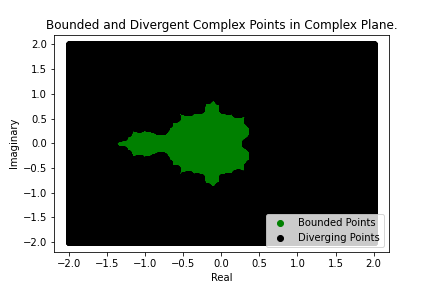
\includegraphics[scale=0.7]{q1_1.png}
    \label{fig:q1_1.png}
\end{figure}
\begin{figure}[!htb]
    \centering
    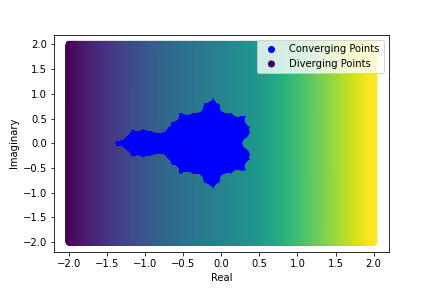
\includegraphics[scale=0.7]{q1_2.png}
    \label{fig:q1_2.png}
\end{figure}
\begin{figure}[!htb]
    \centering
    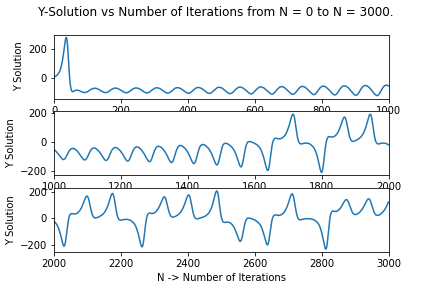
\includegraphics[scale=0.7]{q2_1.png}
    \label{fig:q2_1.png}
\end{figure}
\begin{figure}[!htb]
    \centering
    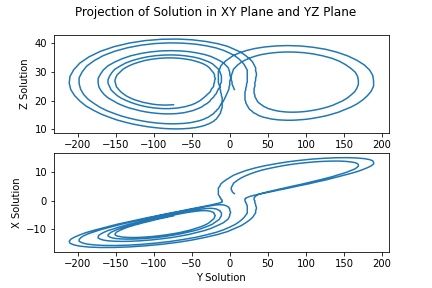
\includegraphics[scale=0.7]{q2_2.png}
    \label{fig:q2_2.png}
\end{figure}
\begin{figure}[!htb]
    \centering
    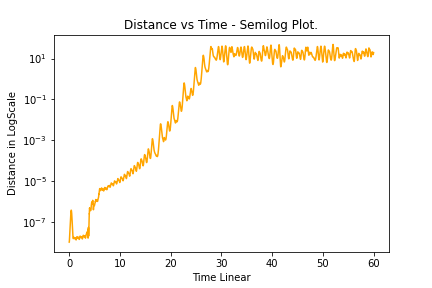
\includegraphics[scale=0.7]{q2_3.png}
    \label{fig:q2_3.png}
\end{figure}



\end{document}